\documentclass[11pt]{article}
\usepackage{geometry}                
\geometry{letterpaper}                 
\usepackage[parfill]{parskip}        
\usepackage{graphicx}
\usepackage{subfigure}
\usepackage{amssymb}
\usepackage{amssymb}
\usepackage{amsmath}
\usepackage{epstopdf}
\usepackage{verbatim}
\usepackage{float}
\usepackage{grffile}
\usepackage{fullpage}
\usepackage{enumerate}
\usepackage{hyperref}
\usepackage[utf8]{inputenc}
\usepackage{gensymb}
\usepackage[T1]{fontenc}
\usepackage[hang,small]{caption}
\DeclareGraphicsRule{.tif}{png}{.png}{`convert #1 `dirname #1`/`basename #1 .tif`.png}

\graphicspath{ {C:/Users/Nate/Documents/School/EECS351/Nates Discussion Material/Discussion 4} }
\usepackage{listings}
\usepackage{color}
\usepackage{textcomp}
\definecolor{listinggray}{gray}{0.9}
\definecolor{lbcolor}{rgb}{1,1,1}
\lstset{
	backgroundcolor=\color{lbcolor},
	tabsize=4,
	rulecolor=,
	language=matlab,
	basicstyle= \scriptsize,
	upquote=true,
	aboveskip={1.5\baselineskip},
	columns=fixed,
        	showstringspaces=false,
        	extendedchars=true,
        	breaklines=true,
        	prebreak = \raisebox{0ex}[0ex][0ex]{\ensuremath{\hookleftarrow}},
        	frame=single,
        	showtabs=false,
        	showspaces=false,
        	showstringspaces=false,
        	identifierstyle=\ttfamily,
        	keywordstyle=\color[rgb]{0,0,1},
        	commentstyle=\color[rgb]{0.133,0.545,0.133},
        	stringstyle=\color[rgb]{0.627,0.126,0.941},
}


\begin{document}

\section*{EECS351 Discussion 4 Problems, 09/26/16}
Nate Sawicki and Alex Ying \newline
Select problems by Mai Le and Kevin Moon


\section{Discrete-domain Basis Sequences}
Let $x[n] = \{\underline{1},1,2,3,5\}$. Represent $x[n]$ in each of the following bases. 

Note: You won't be asked to do anything like this on the homework or exams, but hopefully it will help you solidify your understanding of bases from lecture.

\subsection*{Unit Step Sequences}
Recall $u[n] = \begin{cases}1, & n \geq 0\\ 0, & n < 0 \end{cases}$. Let $\mathcal{S}_u = \{u[n-n_0]|n_0 \in \mathbb{Z}\}$ (unit steps shifted by any integer $n_0$) be your basis sequences. Represent $x[n]$ in $\mathcal{S}_u$.

In other words, show you can write $x[n]=\sum\limits_{k=-\infty}^\infty c_k u[n-k]$ by finding the values for $c_k$.

{\color{blue}
$c = \{\underline{1}, 0, 1, 1, 2, -5\}$
}

\subsection*{Three-Tap Rectangles}
Let $r[n] = \{\underline{1},1,1\}$ and $\mathcal{S}_r = \{r[n-n_0]|n_0 \in \mathbb{Z}\}$. Represent $x[n]$ in $\mathcal{S}_r$.

{\color{blue}
$c = \{\underline{1}, 0, 1, 2, 0, 2, -4, 2, 2, -4, 2, 2, -4, \ldots \}$
}

\subsection*{Three-Tap Triangle}
Let $t[n] = \{\underline{1},2,1\}$ and $\mathcal{S}_t = \{t[n-n_0]|n_0 \in \mathbb{Z}\}$. Represent $x[n]$ in $\mathcal{S}_t$.

{\color{blue}
$c = \{\underline{1}, -1, 3, -2, 6, -10, 14, -18, \ldots \}$
}

\newpage


\section{Graphical Depiction of Change of Basis}
(a) Draw an x and y axis in $ \mathbb{R}^2 $ representing the canonical basis. Represent the signal x = [2 2]$^{T}$ graphically in this basis.
Show that B is orthonormal.\newline
(b) Draw an two axes in $ \mathbb{R}^2 $ corresponding the following basis:


\begin{center}
\[
v_1 = 
\begin{bmatrix}
   1 \\
   0          
\end{bmatrix},
v_2= 
\begin{bmatrix}
   0 \\
   -1          
\end{bmatrix}
\]
\end{center}

(c) Find the coordinates for x = [2 2]$^T$ with respect to the basis from part (b)\newline
(d) Draw a graphical depiction of part (c) on the same axes you used for part (a). Verify that your signal vector is the same for both bases, even though your coordinates/coefficients will be different.

\vspace{4mm}


\begin{figure}[h]
\centering
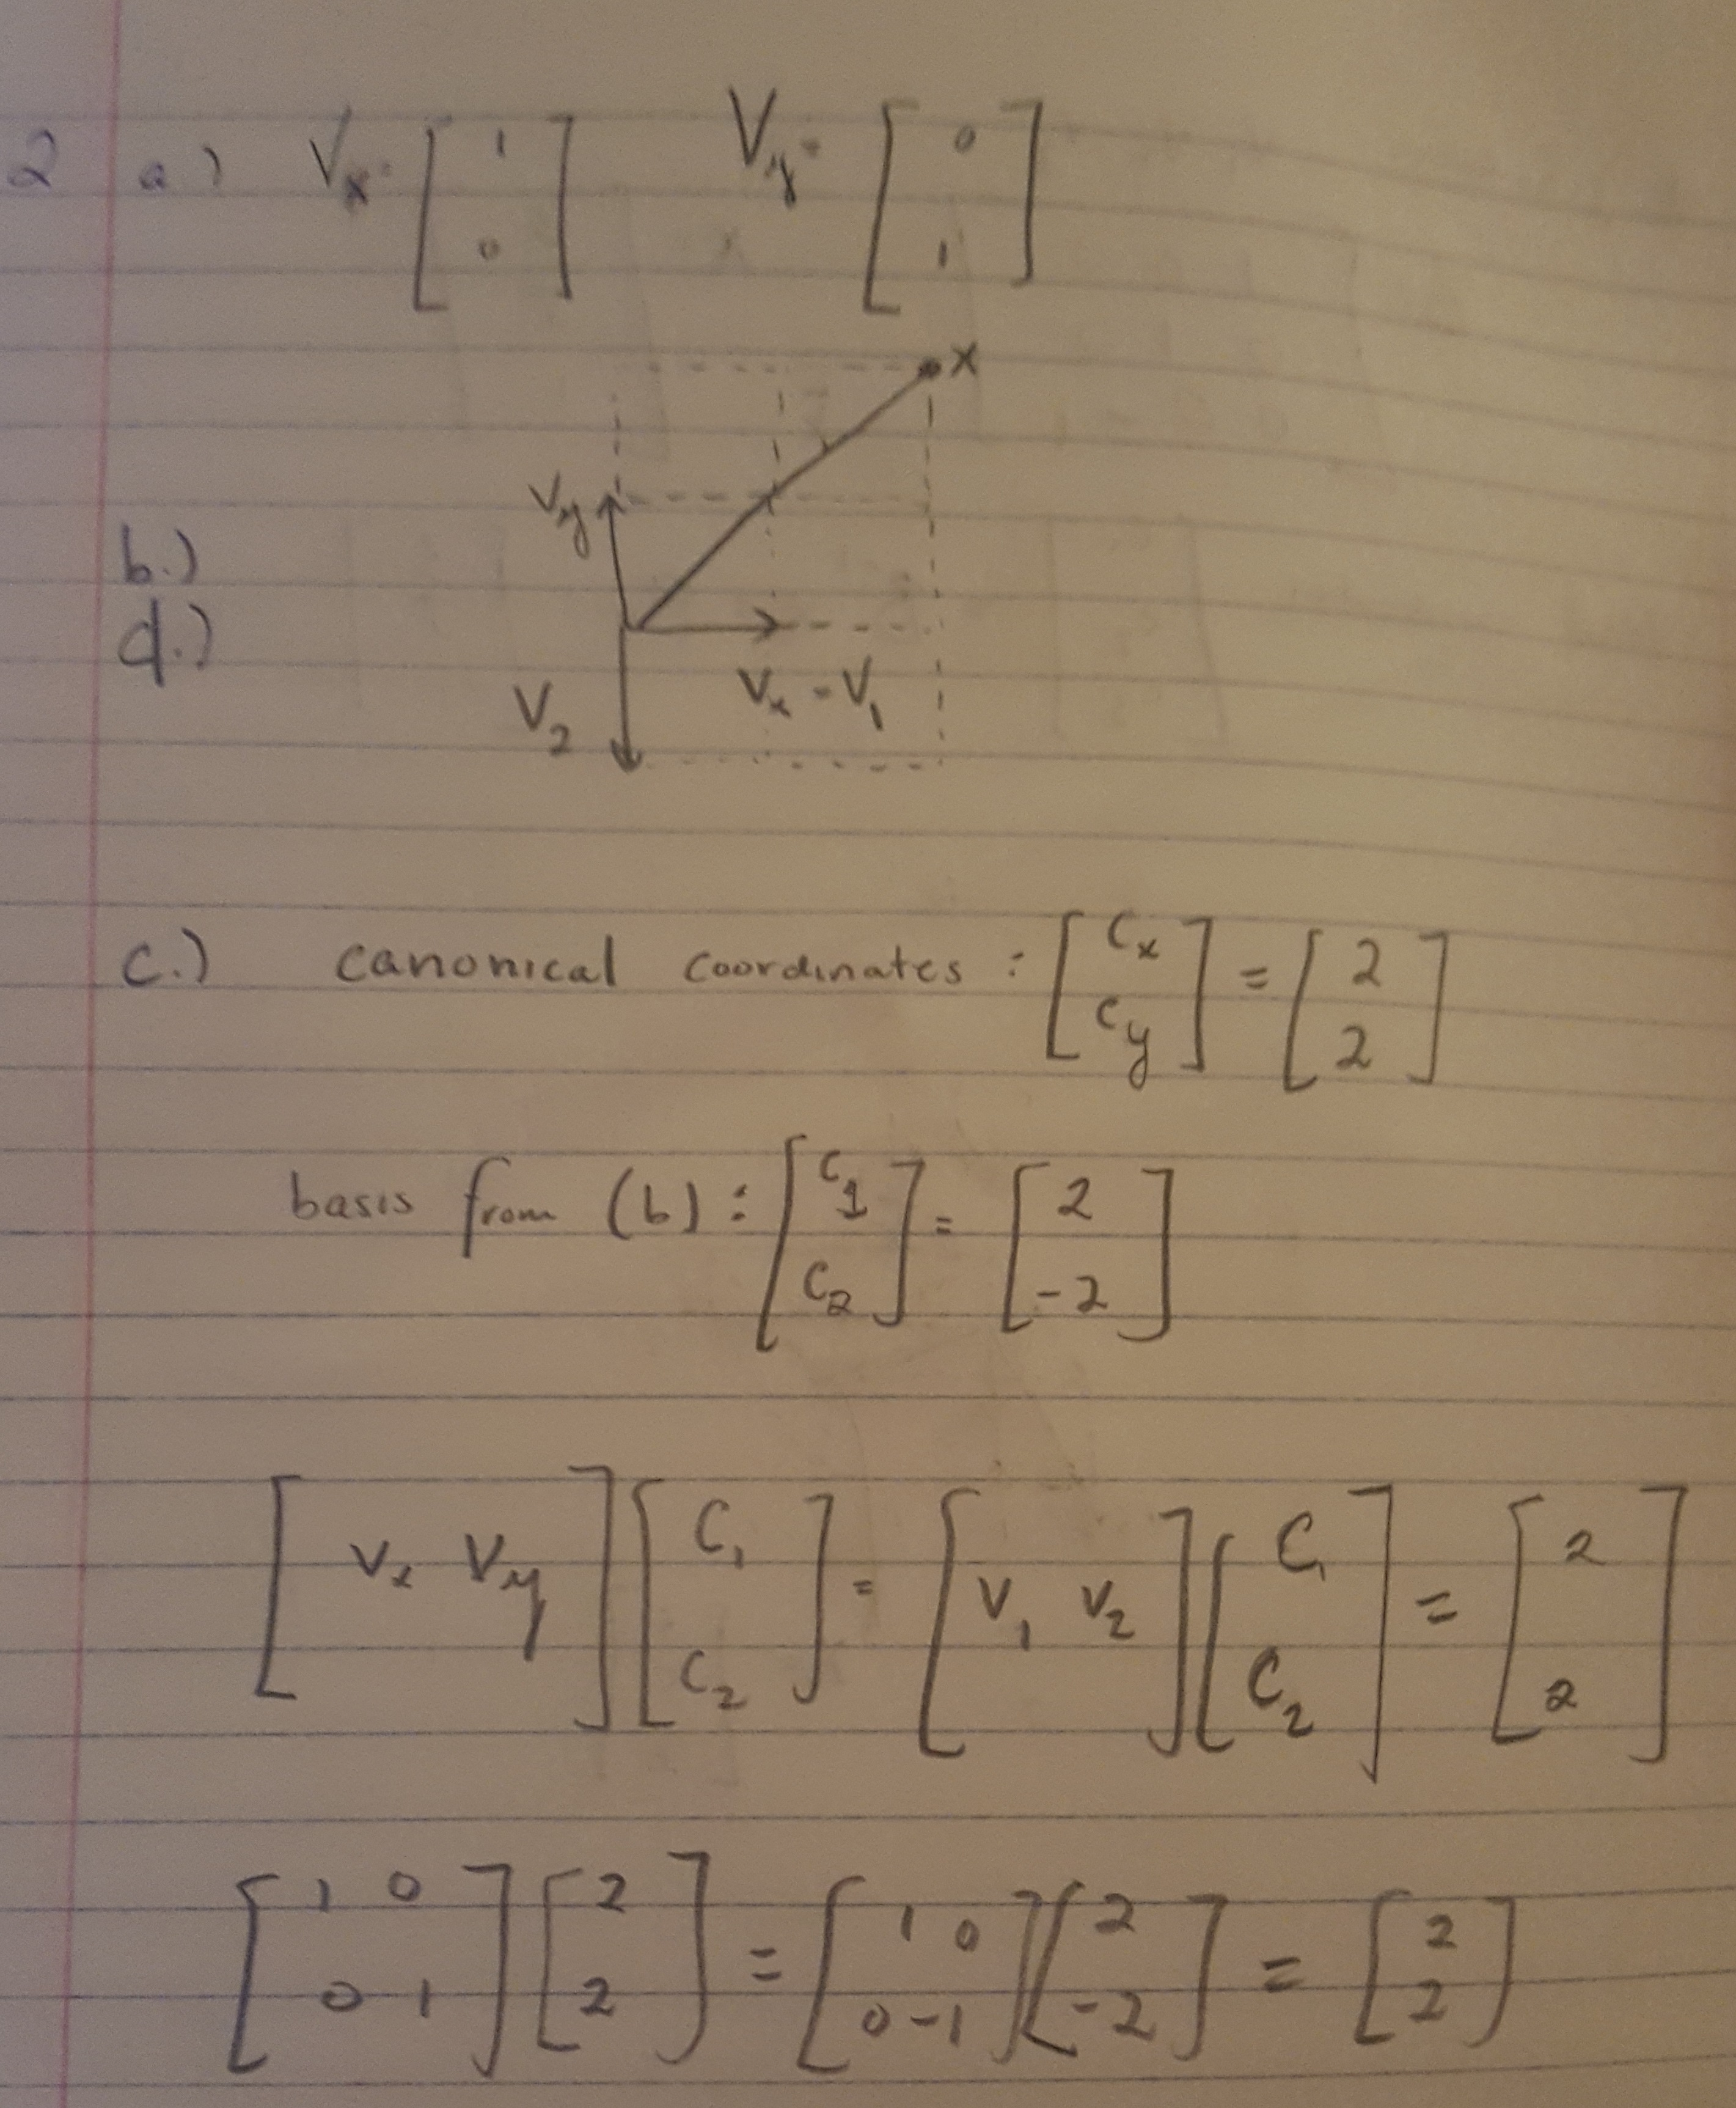
\includegraphics[width=0.6\textwidth]{graphical2d.jpg}
\caption {Coordinates for new basis and canonical basis}
\end{figure}

\newpage

\section{Inner Product}
Show that the Euclidean dot product in $\mathbb{R}^{n}$ satisfies the following conditions of an inner product:\newline

\begin{center}

<x,y> = $\sum_{i = 1}^{n} x_i y_i $

\end{center}

(a) <u + v, w> = <u,w> + <v,w>\newline
(b) <v,v> $\geq$ 0

\vspace{4mm}

{\color{blue}
Solution:\newline
(a) 
\begin{center}

<u+v,w> = $\sum_{i = 1}^{n}(u+v)_i w_i$

\end{center}
\vspace{3mm}
\begin{center}

= $\sum_{i = 1}^{n}(u_i w_i) + \sum_{i = 1}^{n}(v_i w_i)$

\end{center}
\vspace{3mm}
\begin{center}

= <u,w> + <v,w>

\end{center}

(b) 
\begin{center}

<v,v> = $\sum_{i = 1}^{n}(v_i v_i)$

\end{center}
\vspace{3mm}
\begin{center}

= $\sum_{i = 1}^{n}(v_i^2)$ $\geq 0 $

\end{center}

Equality is achieved if $v_i = 0$ for all i


}


\vspace{4mm}
\newpage

\section{$\mathbb{R}^3$}
Express the following signal of length three using any basis \emph{other than the canonical basis} (be sure to use convenient axes):

\begin{center}


\[
x = 
\begin{bmatrix}
   3 \\
   5 \\
   1         
\end{bmatrix}
\]


\end{center}

(b) Graphically depict your answer from part (a)

\newpage

Solution:


\begin{figure}[h]
\centering
\includegraphics[width=0.6\textwidth]{coordinates.jpg}
\caption {Coordinates for new basis}
\end{figure}

\begin{figure}[h]
\centering
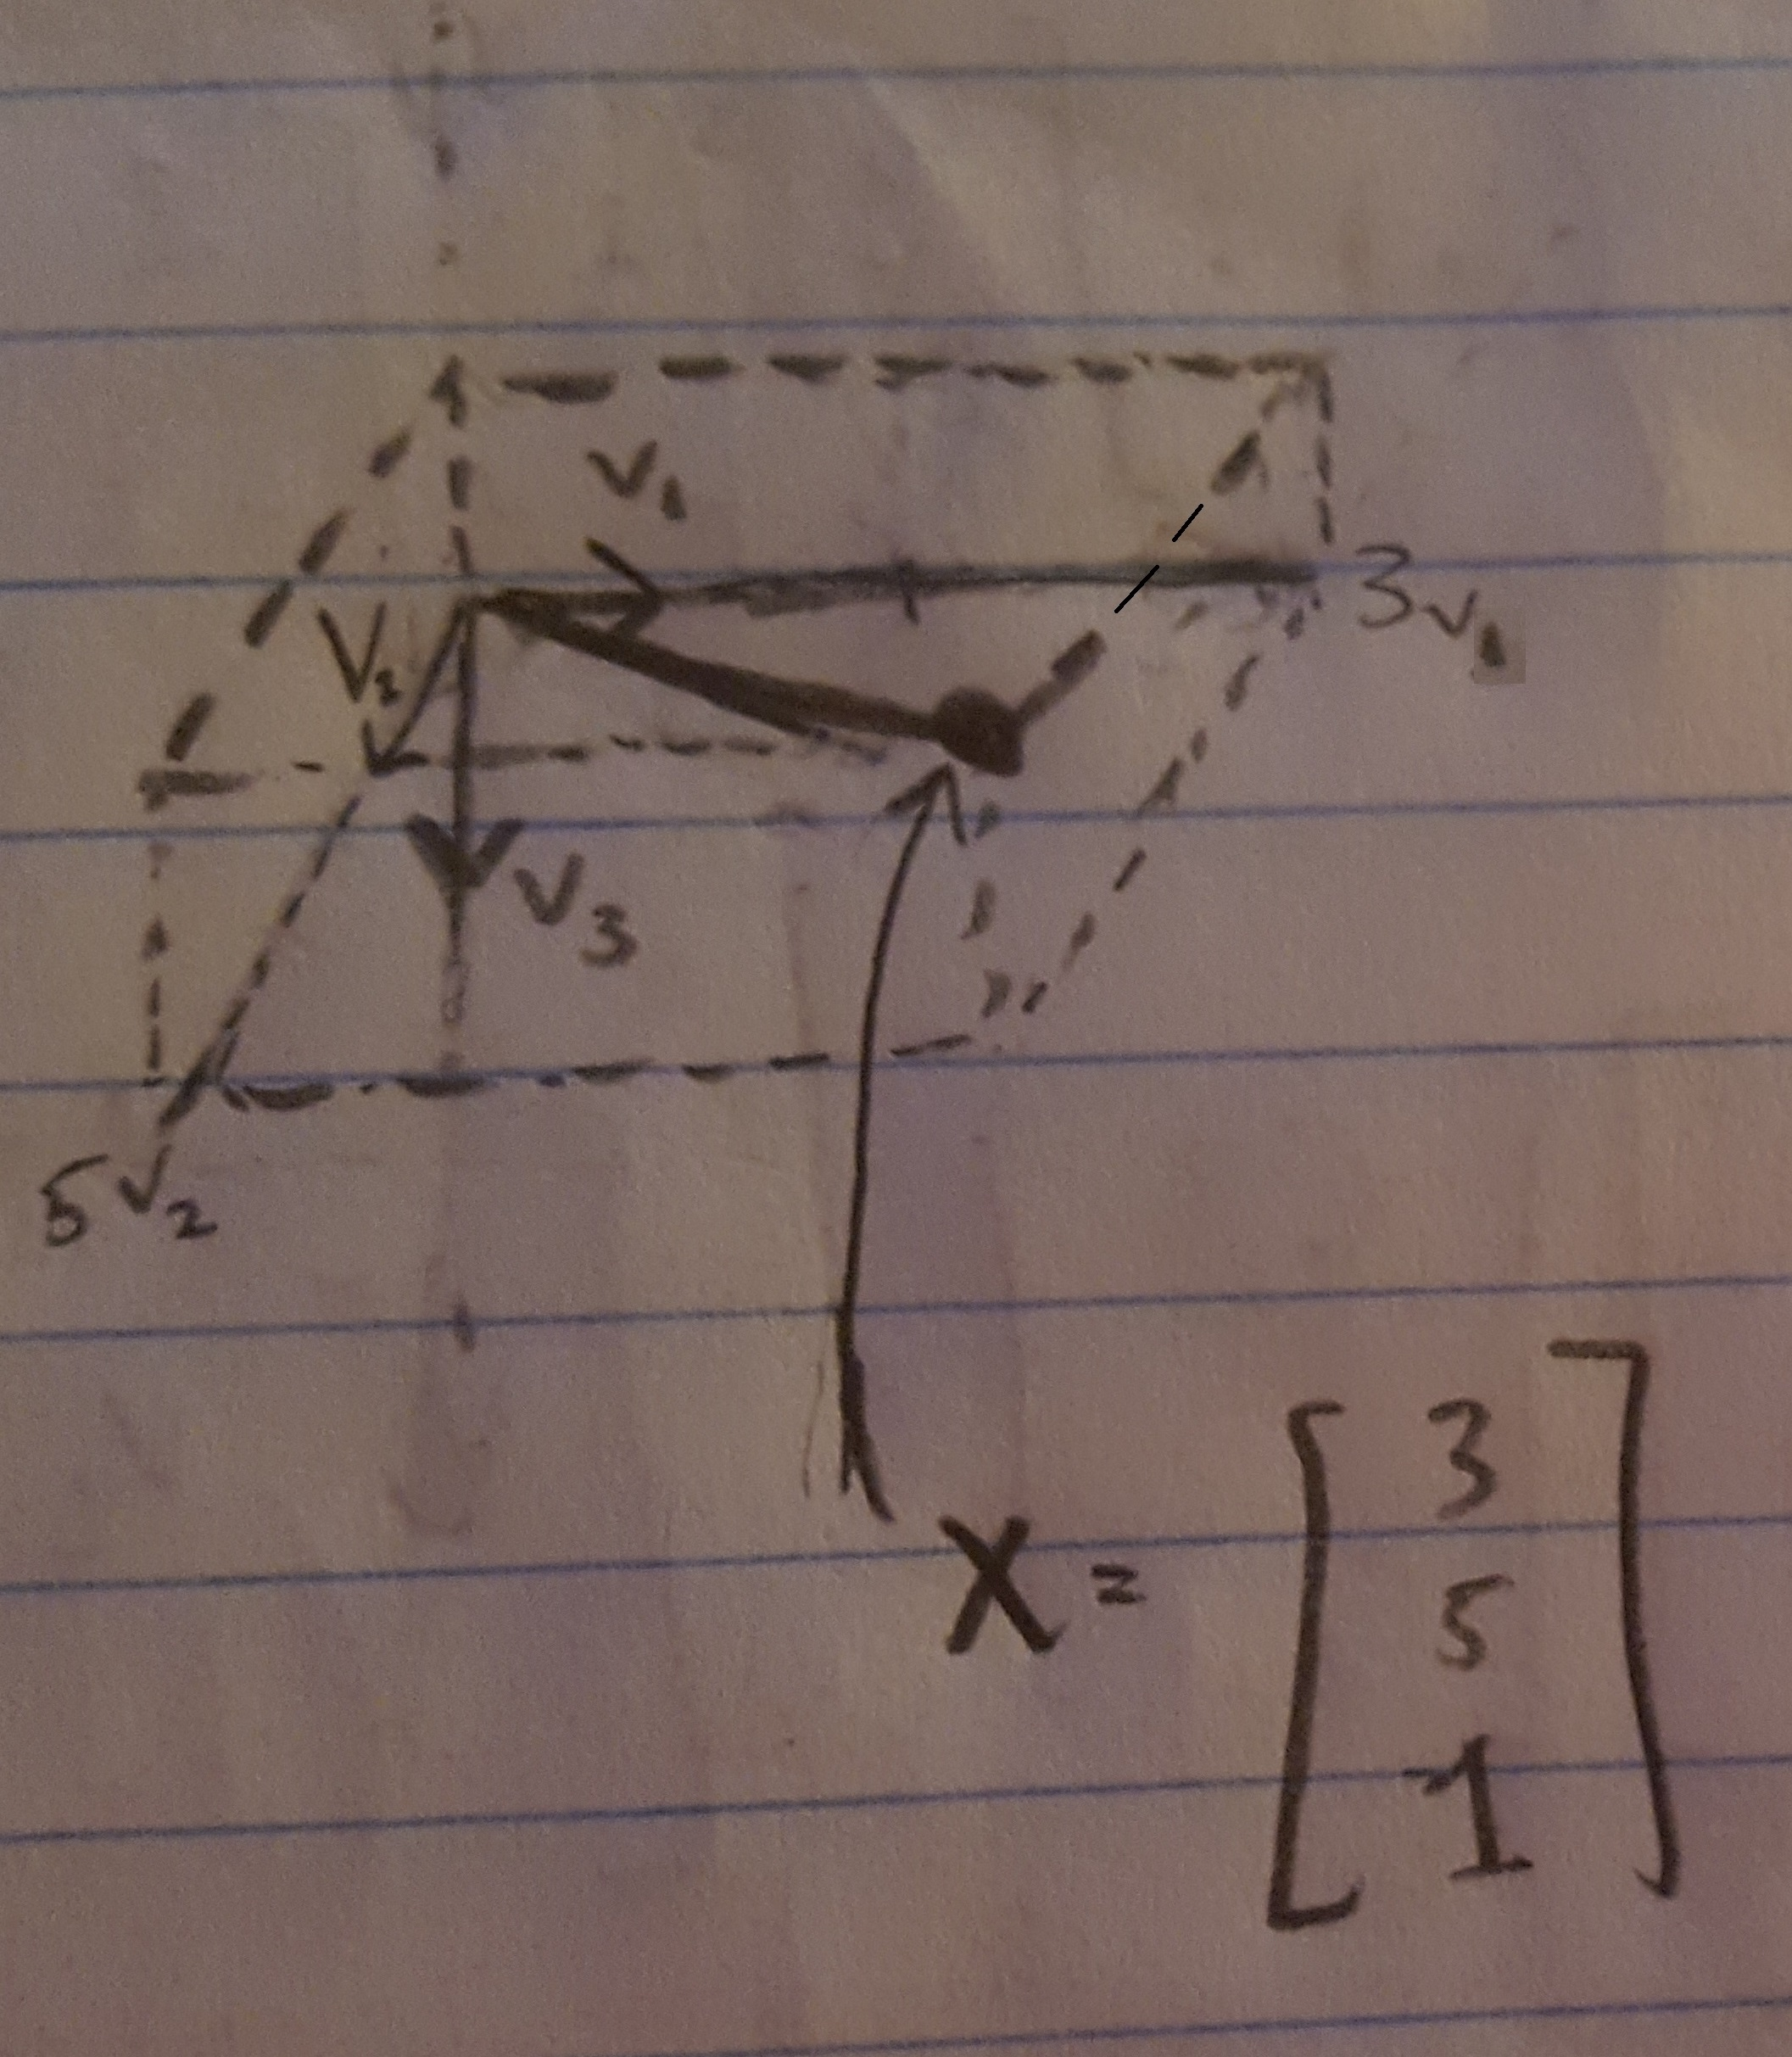
\includegraphics[width=0.4\textwidth]{graphicaldepiction.jpg}
\caption {Draw \textbf{x} onto the new coordinate system}
\end{figure}




\end{document}